\chapter{Medical Dataset}

\section{Overview}

Dane pochodzą z Duke University. Są to zdjęcia z rezonansu magnetycznego głowy wraz z zaznaczonymi obszarami zmian nowotworowych. Obrazy są rozmiaru 256x256x3. Pierwszy kanał jest zdjęciem wykonanym przed wprowadzeniem kontrastu, drugi w trakcie, a trzeci po. Maski mają rozmiar 256x256, a każdy piksel ma wartość 0 albo 255 (255 oznacza komórkę nowotworową). Na rysunku \ref{fig:medical_description} pokazane są osobne kanały oraz maska.

\begin{figure}[h!]
    \centering
    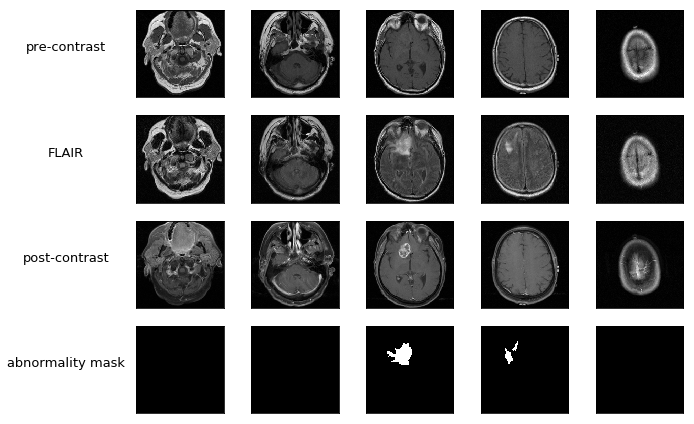
\includegraphics[width=0.8\textwidth]{images/medical_description}
    \caption{}
    \label{fig:medical_description}
\end{figure}

Dane pogrupowane są dla 110 pacjentów. Zestaw dla jednego z nich znajduje się na rysunku \ref{fig:medical_sample}. Łącznie znajduje się 3929 par obrazów, z czego w 1373 jest przynajmniej jedna komórka nowotworowa ($\sim$34.95\%). Natomiast w całym zbiorze piksele oznaczające zmiany nowotworowe stanowią jedynie $\sim$1.02988\% wszystkich pikseli. Przy tak znaczącej dysproporcji ciężko liczyć na rzetelne podejście supervised, dlatego będę chciał spróbować podejścia unsupervised.

\begin{figure}[h!]
    \centering
    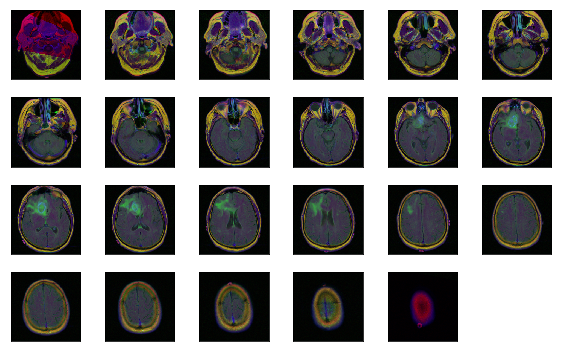
\includegraphics[width=0.8\textwidth]{images/medical_sample}
    \caption{}
    \label{fig:medical_sample}
\end{figure}

\section{Preprocessing}

Opis preprocessingu

\section{Patches}

Wybór rozmiaru patchy i ekspeymenty z tym związane

\section{Normalizations}

\todo{Może LIME?}
